\chapter{Introducci\'on}\label{cap1}

\section{Motivaci\'on}
Actualmente, las herramientas de  modelado gráficas  y automáticas que asisten a los  modeladores son esenciales  debido al incremento  en la complejidad de los sistemas de información. Una mala disposición gráfica de los elementos del  diagrama en el modelo hace que sea difícil de leerlo y de comprenderlo en forma inmediata \cite{Sto14,Sto11,Huang07,ware02}.
	
	Los algoritmos de layout automáticos permiten el reordenamiento de los  elementos gráficos de los diagramas de modelado, de manera que se disponga una visualización más satisfactoria de los mismos, como puede verse en la Figura \ref{fig:ejemplo_crossnum}.
	Sin embargo, por estar basados en problemas de optimización combinatorios, heredan la  complejidad computacional de éstos,  que en su mayoría  son  NP-Completos \cite{Papadimitriou1976, Garey:1974}. 
	
	\begin{figure}[h]
		\centering
		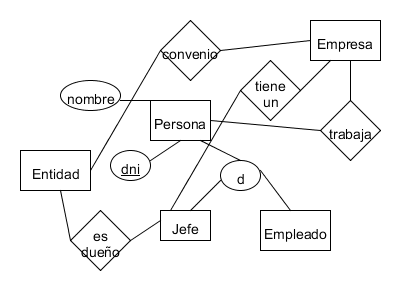
\includegraphics[width=5cm]{imagenes/ejemplo_malo.png}
		\hspace{1.5cm}
		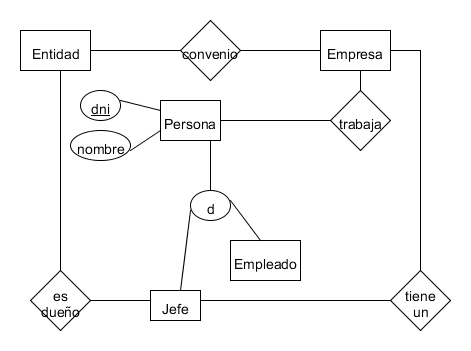
\includegraphics[width=5cm]{imagenes/ejemplo_bueno.png}
		\caption{Dos formas de dibujar un diagrama ER. El primer diagrama presenta 3 cruces, y no resuelve una disposición geométrica de los elementos, en cambio el segundo mejora estos aspectos.}
		\label{fig:ejemplo_crossnum}
	\end{figure}
	
	
	
	%	 A good drawinq is one in which no two arcs incident with a common node have a common point, and no two arcs have more than one point in common.
	
	%Para este trabajo se plantea un algoritmo que recibirá como entrada un modelo conceptual expresado en diferentes lenguajes como UML, ER, ORM, etc, y se buscará un
	
	En este trabajo se introduce un nuevo algoritmo  genético,  denominado \textsc{ArcGen},  que es el  punto de partida  para  resolver el problema de la correcta visualización de un modelo conceptual expresado en UML o  ER  y que será incorporado a {\it Crowd} \cite{gimenez2016crowd}. {\it Crowd} es una herramienta web para modelado ontológico utilizando los lenguajes  UML \cite{booch2005unified}\ y  ER \cite{chen1988entity}, con soporte de razonamiento para asistir al usuario en tareas de diseño y validación. 
	
	En esta primer etapa,  nos centramos en la resolución del problema de Crossing Number, motivados por la  importancia  estética de reducir el número de cruces de arcos en la representación gráfica de grafos \cite{Kob14}. Este es un problema NP-Completo \cite{garey1983crossing} de gran importancia para la visualización de grafos, que radica en evitar, en la mayor medida posible, que los arcos de un grafo dibujado sobre el plano Euclídeo se crucen.
	%de manera que se obtenga un grafo con menos puntos de  cruces de arcos  respecto del grafo original. 
	Asimismo, circunscribimos la solución que se propone  a grafos con ciertas características encontradas en los diagramas de modelado conceptual (tamaño y complejidad).
	
	% de grafos de entrada, es decir, que obtendrá un resultado eficiente considerando parámetros normales de entrada.
	
	El algoritmo \textsc{ArcGen} involucra un preprocesamiento del grafo original,  transformando su representación a una  forma particular, llamada Diagrama de Arcos \cite{saaty1964minimum} o Linear Embedding \cite{masuda1990crossing} según las diferentes fuentes. Un Diagrama de Arcos \cite{Wat02,Nich68,saaty1964minimum}\ es una representación de  un grafo en un plano, donde los nodos se ubican sobre una recta, como puede visualizarse en la Figura \ref{fig:arcdiagram_k6_no_optimo}. Esta representación del grafo tiene la cualidad de %no generar cruces de arcos provocados por la representación, si no, 
	que los cruces obtenidos dependerán del ordenamiento de los nodos, esto es, su disposición sobre la línea y del  semiplano en el que se  dibuja el arco, es decir, como un semicírculo por arriba de la recta o por debajo de ella. %Por lo tanto, esta representación nos facilita el desarrollo de un algoritmo para la resolución parcial de Crossing Number.
	Inicialmente, se trabajó sobre grafos completos \cite{Aich02}, buscando un ordenamiento de sus nodos que generen un número mínimo de cruces de arcos.
	%Dada esta forma gráfica de un grafo, se propone en un principio buscar un ordenamiento para permitir que grafos completos (aquellos en que cada par de nodos está conectado por un arco) dispongan de un número de cruces de arcos mínimo.
	Este problema se ha podido solucionar satisfactoriamente con un algoritmo simple, permitiendo cumplir con la cota superior dada por la conjetura de Guy \cite{guy1960combinatorial}. %, como se verá en la sección \ref{sec:arcdiagram}.
	Sin embargo,  al utilizar este algoritmo sobre grafos no completos, las  mejoras obtenidas en el número de cruces no fueron suficientes, lo que dió génesis a {\sc ArcGen}.
	
	La  población inicial de {\sc ArcGen}  está generada a partir de la representación Diagrama de Arcos mejorada del  grafo original, lo que guía la búsqueda del menor número de cruces.%, explicado en la sección \ref{sec:genetico}.
	
	Los resultados experimentales realizados sobre grafos no dirigidos de tamaño moderado muestran que  {\sc ArcGen} se comporta en forma satisfactoria, disminuyendo en algunos casos hasta en 4 veces la cantidad de cruces sobre la representación original. 
	%\todo[inline, color=green]{Creo que habria que agregar un párrafo  de otras herramientas que analizaste y marcar diferencias. Diferencia con otros es que la  población inicial del  algoritmo genético parte de un grafo preprocesado.}
	
	Existen otros  algoritmos genéticos que resuelven el problema, como  TimGA \cite{eloranta2001timga}\ el cual, a diferencia del algoritmo \textsc{ArcGen}, propuesto en este trabajo, utiliza grafos genéricos para la representación de sus individuos, almacenando las posiciones $x$ e $y$ de cada nodo en matrices y considerando la representación gráfica de los arcos como rectas entre tales nodos. Esta representación produce gran cantidad de variaciones y posibles grafos, haciendo que el algoritmo genético deba realizar mayor cantidad de generaciones, además de no permitir la representación de arcos curvos. De esta manera, genera implícitamente mayor cantidad de cruzamientos. 
	
	Por otro lado, el propuesto por Hongmei He et al. \cite{he2007parallelisation}\ considera la representación  Diagrama de Arcos, pero comienza con una población generada aleatoriamente a diferencia de \textsc{ArcGen} que genera la población a partir de un individuo dado por el algoritmo de grafos completos. Esto causa que el algoritmo consuma más tiempo en alcanzar un máximo local o global, quitándole practicidad para el objetivo buscado.
	
	En el survey de Helen Gibson et al. \cite{gibson2013survey} se han recopilado gran variedad de algoritmos de layout, de los cuáles el más adecuado, con respecto a precisión y velocidad, para layout en modelado conceptual, es el algoritmo Dirigido por Fuerzas de Tunkelang \cite{tunkelang1998jiggle}. Este algoritmo  propone un modelo físico donde los nodos y arcos realizan fuerzas de repulsión entre ellos para evitar cruzamientos. Esta simulación se realiza por un tiempo dado hasta obtener el resultado deseado. Tal algoritmo no consigue la precisión que se busca, debido a que la eficacia del resultado está ligada a las posiciones iniciales del grafo de entrada. %, por lo que se consideró abordar el problema desde un modelo jerárquico, el cual consta de un reordenamiento de posiciones fijas, tal como se realiza en los algoritmos genéticos mencionados anteriormente.
	
	Este trabajo está organizado de la siguiente manera. En la sección 	\ref{sec:arcdiagram},  se propone un algoritmo  que esquematiza  un grafo arbitrario en un Diagrama de Arcos optimizado para grafos completos. En la sección \ref{sec:genetico}, se explica el algoritmo genético desarrollado para minimizar la cantidad de cruces de arcos  respecto del  grafo original. Luego en la sección \ref{sec:implementacion}, se describe la aplicación que genera el grafo optimizado. En la sección \ref{sec:resultados}, se presentan resultados experimentales realizados  sobre la aplicación. Finalmente, se presentan las conclusiones y trabajos futuros.

\section{Objetivos}

El objetivo general de este trabajo es el diseño e implementación  de un algoritmo de layout automático de grafos para la visualización en herramientas de modelado conceptual. Se pretende trabajar en un diseño que utilice técnicas de Inteligencia Artificial y que  permita adaptar las funcionalidades de visualización de los diagramas, considerando los diferentes lenguajes de modelado conceptual, como EER, UML y \mbox{ORM 2.}
Se espera que los expertos o modeladores puedan utilizar tales herramientas de acuerdo a sus preferencias de notación con una disposición apropiada de los elementos visuales de los lenguajes de modelado conceptual, lo que redituará en una mejor legibilidad y un adecuado entendimiento del diagrama, potenciando la comunicación entre los interesados en la información del modelo.



\subsection{Objetivos Específicos}

\begin{itemize}
\item Analizar e identificar las cualidades que debe tener la disposición de un grafo, para que su visualización sea  satisfactoria.%, como también relevar las técnicas de layouts automáticos para grafos ya existentes.

\item Diseñar un algoritmo que permita realizar layout automático con técnicas de Inteligencia Artificial, orientado a su aplicación específica en modelado conceptual y que cumpla con las cualidades identificadas.
\item Implementar un prototipo de dicho algoritmo.% de manera que pueda ser integrado en herramientas de modelado conceptual como {\it Crowd}\cite{gimenez2016crowd}.

\end{itemize}
% \section{Contribuciones}

% \section{Estructura de la Tesis}
